%KOMA-script
%\documentclass[]{report}

\documentclass[]{report}
%\usepackage[english, ku, titlepage]{ku-frontpage}
%\usepackage[utf8]{inputenc}
\usepackage[acronym]{glossaries}
\usepackage{multirow}
\makeglossaries
%opening
%\assignment{Master Thesis}
\title{LC-MS based Metabolomics: Biomarker Discover and Bioinformatics Tools}
\author{Tu Hu\thanks{Supervised by Lars Ove Dragsted and Gözde Gürdeniz}}
%\subtitle{Examplified by Whole Grain Barley, Wheat Intake and FATMAD}
%\advisor{Supervisor: Lars Ove Dragsted \& Gözde Gürdenz}
\date{Sep, 2019}
\usepackage[backend=biber,style=nature,%sorting=ynt
]{biblatex}
%\usepackage{glossaries}
\addbibresource{barley.bib}
\usepackage{tabularx}
\usepackage{graphicx}

\usepackage{siunitx}
\usepackage{gensymb}
\usepackage[backend=biber,style=nature,%sorting=ynt
]{biblatex}


\usepackage{makecell}
\usepackage{footnote}
\usepackage{lscape}
\newacronym{cvd}{CVD}{cardiovascular diseases}
\newacronym{tc}{TC}{Total Cholesterol}
\newacronym{ldlc}{LDL-C}{Low Density Lipoprotein Cholesterol}
\newacronym{hdlc}{HDL-C}{High Density Lipoprotein Cholesterol}
\newacronym{tg}{TG}{Triglycerides}
\newacronym{crp}{CRP}{C-Reactive Protein}
\newacronym{wbb}{WBB}{Whole Barley Bread}
\newacronym{wwb}{WWB}{Whole Wheat Bread}
\newacronym{bfis}{BFIs}{Biomarkers of Food Intake}
\newacronym{lc-ms}{LC-MS}{Liquid Chromatography-Mass Spectrometry}
\newacronym{gc-ms}{GC-MS}{Gas Chromatography-Mass Spectrometry}
\newacronym{nmr}{NMR}{Nuclear Magnetic Resonance Spectroscopy}
\newacronym{ms/ms}{MS/MS}{Tandem Mass Spectrometry}
\newacronym{tims-pasef}{TIMS-PASEF}{Trapped Ion Mobility Spectrometry with Parallel Accumulation Serial Fragmentation}
\newacronym{hmdb}{HMDB}{Human Metabolome Database}
\newacronym{gnps}{GNPS}{Global Nature Products Social Molecular Networking}
\newacronym{aw}{AW}{After Wheat}
\newacronym{ab}{AB}{After Barley}
\newacronym{bw}{BW}{Before Wheat}
\newacronym{bb}{BB}{Before Barley}
\newacronym{pca}{PCA}{Principle Component Analysis}
\newacronym{plsda}{PLSDA}{Partial Least Squares Discriminant Analysis}
\newacronym{pqn}{PQN}{Probabilistic Quotient Normalization}
\newacronym{vip}{VIP}{variable importance in projection}
\usepackage{siunitx}

\usepackage{pdfpages}
\begin{document}
\maketitle
%% abstract
%\begin{abstract}
%	This calls for an abstract.
%\end{abstract}
%% table of content
\tableofcontents

\newacronym{cvd}{CVD}{cardiovascular diseases}
\newacronym{tc}{TC}{Total Cholesterol}
\newacronym{ldlc}{LDL-C}{Low Density Lipoprotein Cholesterol}
\newacronym{hdlc}{HDL-C}{High Density Lipoprotein Cholesterol}
\newacronym{tg}{TG}{Triglycerides}
\newacronym{crp}{CRP}{C-Reactive Protein}
\newacronym{wbb}{WBB}{Whole Barley Bread}
\newacronym{wwb}{WWB}{Whole Wheat Bread}
\newacronym{bfis}{BFIs}{Biomarkers of Food Intake}
\newacronym{lc-ms}{LC-MS}{Liquid Chromatography-Mass Spectrometry}
\newacronym{gc-ms}{GC-MS}{Gas Chromatography-Mass Spectrometry}
\newacronym{nmr}{NMR}{Nuclear Magnetic Resonance Spectroscopy}
\newacronym{ms/ms}{MS/MS}{Tandem Mass Spectrometry}
\newacronym{tims-pasef}{TIMS-PASEF}{Trapped Ion Mobility Spectrometry with Parallel Accumulation Serial Fragmentation}
\newacronym{hmdb}{HMDB}{Human Metabolome Database}
\newacronym{gnps}{GNPS}{Global Nature Products Social Molecular Networking}
\newacronym{aw}{AW}{After Wheat}
\newacronym{ab}{AB}{After Barley}
\newacronym{bw}{BW}{Before Wheat}
\newacronym{bb}{BB}{Before Barley}
\newacronym{pca}{PCA}{Principle Component Analysis}
\newacronym{plsda}{PLSDA}{Partial Least Squares Discriminant Analysis}
\newacronym{pqn}{PQN}{Probabilistic Quotient Normalization}
\newacronym{vip}{VIP}{variable importance in projection}



\printglossaries
%\newpage

%\addchap{Preface}
%\addchap{Introduction}
%\section{Biomarker Discovery}
\subsubsection{Definition of Biomarker}


\subsubsection{Biomarker Classification}


\subsubsection{Biomarker Systematic review}
\textbf{Credibility of BFIs}: Putative biomarker, Candidate biomarker, partially validated biomarker and fully-validated biomarker

\subsubsection{Biomarker Validation}



%\chapter{Introduction}
%%\subsection{R, Tidy Format and Data Wrangling}
%R is an open-source data analysis language.
%R is perfect for bioinformatics analysis.
%Tidy format is a term used in R describing a philosophy of storing data. Tidy format has the characteristics:
%\begin{itemize}
%	\item each variable is in its own column
%	\item each observation, or case, is in its own row
%\end{itemize}
%If data is stored in tidy form. Data scientists spend less time fighting with the tools and more time working on your analysis.


\subsection{Statistics method}
\subsubsection{Comparisions between Univariable and Multivariable statistics}
t-test has multiple testing problem. because when we do a t-test, normally we use a cutoff value of 0.05, it also means we take the risk of 5\% probability that it's NOT significantly different, but classified as different. this is called multiple testing problem. 

FALSE DISCOVERY problem in metabolomics.

how to overcome this problem? adjusted t-test, or reduce the cutoff to a reasnable value.

multivariable data analysis and univariable data analysis show different aspects of data. It is very common to observe analysis results are significant univariablely but not multivaribalely, also, it is common to see that another way. This means uni-/multi- variable data analysis both have their limitations. that's why it is recommanded that do both uni and multi variable data analysis for the same dataset.

However, how to integrate these analysis? are they chemically correlated? maybe one feature significant in univariable analysis is associated with another one in multivaribale data analysis? Maybe, one way is to first merge all these results together. in addition, because based on current technology limitation, it's impossible to identify OR intereprete all Metabolomics results, actually also time and resources. it actually exists priorities in identifying. better chance to identify, if they're correlated. meanwhile, if intensities are high.


\subsection{Identification}
\subsubsection{Level of Identification and communication confidence}
Reporting level of identification together with identification results can enhance communication confidence. Identification is recognized by far the most difficult part of Metabolomics research, especially concerning novel compound or biomarker discovery. 

In a single research project, not all structures or chemical information could be confirmed. Therefore, besides reporting chemical information (such as mass and structures), it is equally important to report the confidence of identification.

Five levels of confidence were proposed and applied extensively in xxx areas of LC-MS based compound identification\cite{?}.

\subsection{Validation of the Biomarker}



%\newpage
%\section{Materials and methods}
%\subsection{A mini-systematic literature review of whole grain wheat and barley intake biomarkers}
A systematic literature review of whole grain wheat and barley intake biomarkers was conducted. This will prioritize future work on the identification of new potential biomarkers and on validating them.

The mini-review referred '8-step' Biomarker of Food Intake Reviews (BFIRev) Guidelines \cite{Pratico2018}.

%ISI Web of Science
\subsubsection{Designing the review for whole grain wheat and barley}
The \textbf{objective} of this review is to identify and evaluate reported biomarkers for dietary assessment of whole grain wheat and barley.

\subsubsection{Searching for relevant BFI research paper}
Keywords used for searing BFI barley in human: 
(barley) AND (biomarker* OR marker* OR metabolite* OR biokinetics OR biotransformation OR pharmacokinetics) AND (intake OR meal OR diet OR ingestion OR consumption OR eating OR food) AND 
(human* OR men OR women OR patient* OR volunteer* OR participant*) AND 
(trail* or experiment OR study) AND (urine OR plasma OR blood OR serum OR excretion OR hair OR toenail OR faeces OR faecal water)

Keywords used for searing BFI barley in animals: 
(barley) AND (biomarker* OR marker* OR metabolite* OR biokinetics OR biotransformation OR pharmacokinetics) AND (intake OR meal OR diet OR ingestion OR consumption OR eating OR food) AND 
(animal* OR goat OR sheep OR cow OR mice OR mouse*) AND 
(trail* or experiment OR study) AND (urine OR plasma OR blood OR serum OR excretion OR hair OR toenail OR faeces OR faecal water)

Keywords used for searing BFI wheat in human: 
(wheat) AND (biomarker* OR marker* OR metabolite* OR biokinetics OR biotransformation OR pharmacokinetics) AND (intake OR meal OR diet OR ingestion OR consumption OR eating OR food) AND 
(human* OR men OR women OR patient* OR volunteer* OR participant*) AND 
(trail* or experiment OR study) AND (urine OR plasma OR blood OR serum OR excretion OR hair OR toenail OR faeces OR faecal water) since 2008

\subsubsection{Selecting and screening papers for quality and relevance}
The title and abstract were readed in order to remove irrelevant literatures.

\subsubsection{Selection of candidate BFIs and data collection from the included records}

\subsubsection{Assessing quality of included papers on candidate BFIs}


\subsubsection{Evaluating the current overall status of BFIs for the food in question}


\subsubsection{Presenting data and results}


\subsubsection{Interpretation and conclusion}

\subsection{Software}
Several software packages were used for different purposes.

MATLAB R2018a (9.4.0.813654) coupled with PLS toolbox was used for data processing, modeling.

MZmine 2.31, an open source data processing software for \acrshort{lc-ms} and \acrshort{gc-ms}. 

MassLynx was used to check mass spectra.

DataBridge, an \acrshort{lc-ms} data file conversion program built-in MassLynx developed by Waters.

XCMS Online was used for uni-variable data analysis.


\subsection{Data-preprocessing}
Data-preprocessing consists x steps.

% Data convertion
First, data format was converted by DataBridge from '.raw' to '.cdf'. '.raw' was the format directly generated by Waters analytical platform. In order to be readable by MZmine, data was converted\footnote{N.B. Although in MZmine manual, '.raw' file is described as a compatible format, in practice some weird errors were generated when '.raw' format was input into MZmine.}.

% MZmine step
Then, the data was preprocessed by MZmine (2.31) following the steps: peak detection, deisotoping, alignment and gap filling.

Positive mode and negative mode were separately processed because of different noise level and in-source reaction. Blank samples were also excluded in pre-processing.

% result
In the end, the detected features, including information of mass to charge ratio (m/z), retention time (rt) and intensities were output as '.csv' files for further investigation.

%XCMS
%\subsection{Data conversion from MATLAB to R}
%'m2r.R'\footnote{codes were reposited on GitHub: https://github.com/tuhulab/bfi-wholegrain/blob/master/r/m2r.R} can convert a matlab dataset into R tidy form.

\subsection{Statistics}
\subsubsection{Paired t test}
Paired-t test and unpaired-t test were conducted on XCMS Online (xcmsonline.scripps.edu).

\subsection{PCA}
PCA was used for quality control and outlier detection.

\subsection{PLSDA modeling}
PLSDA modeling was used to select variables that have significant differences. 

\subsection{Literature search}
using qian's article as a reference


%\section{Results}
%\subsection{Mini-systematic literature review of whole grain wheat and barley intake biomarkers}

\begin{tabular}{|c|c|c|c|c|c|c|}
	\hline 
	Type of WG & No. subjects  & Sample type  & Analytical method & Enzymatic hydrolysis & Candidate biomarker & Reference \\ 
	\hline 
	WG wheat and rye & 40 & 24-h spot urine &  &  & DHCA, DHBA-glycine, DHPPTA & \\ 
	\hline 
	&  &  &  &  & & \\ 
	\hline 
	&  &  &  &  & & \\ 
	\hline 
	&  &  &  &  & & \\ 
	\hline 
	&  &  &  &  & & \\ 
	\hline 
	&  &  &  &  & & \\ 
	\hline 
\end{tabular} 


\subsection{Unpaired t-test of Negative Mode Urine Samples}
\begin{tabular}{c|c|c}
	hi | hi
\end{tabular}

\subsection{PLSDA modelling to select variables of plasma samples}
For serum data, plsda modelling can not select any significant features to distinguish after wheat and after barley intervention groups.

Possible reasons could be:
* because plasma samples were fasting plasma samples. Metabolites were already excreted.


\subsection{Alkylresorcinol metabolites in plasma and urine samples}
Three alkylresorcinols metabolites were detected. 
%\section{Conclusions}
%Limitation of LC-MS based metabolomics BFIs discovery: 
(1) instruments and their maintainance plus the analytical method development and optimization are expensive.
(2) it always involves clinical or human trail. it is expensive, time and energy consuming
(3) knowledge of researchers: chemistry, food science, nutritional science, human physiology, data analysis and programming is needed.

Metabolites are fluctuating.
 


%\newpage
%\section{Appendix}
%\subsection{Chromatogram of Barley Flour}
\begin{figure}[h]
    \centering
    \includegraphics[scale=0.4]{images/chromatogram_barley_1.png}
    \caption{Chromatogram of Barley Flour (from top to the bottom: bran flour and endosperum flour)}
    \label{fig:chromatogram_barley}
\end{figure}

\clearpage
\subsection{\acrfull{ms/ms} spectra of phytosterols}
\acrshort{ms/ms} spectra of common phytosterols are shown in Figure \ref{fig:sterolmsms}, adapted from \cite{sterolms}
\begin{figure}[H]
    \centering
    \includegraphics[scale=1]{images/sterolmsms.jpg}
    \caption{\acrshort{ms/ms} spectra of common phytosterols}
    \label{fig:sterolmsms}
\end{figure}
\chapter{Introduction}
\section{Biomarker Discovery}
\subsubsection{Definition of Biomarker}


\subsubsection{Biomarker Classification}


\subsubsection{Biomarker Systematic review}
\textbf{Credibility of BFIs}: Putative biomarker, Candidate biomarker, partially validated biomarker and fully-validated biomarker

\subsubsection{Biomarker Validation}

\chapter{A Mini-review on Biomarkers of Whole Grain Wheat and Barley Intake}
	%\includepdf[pages=-]{review-main.pdf}
	\section{Abstract}
	Due to lacking objective food exposure measurement, epidemiologic studies showed mixed results on whole grains' health beneficial effects.
	Meanwhile, increasing evidence showed each whole grain type could benefit health differently. 
	In order to accurately quantify whole grain exposure, there is a demand to discover intake biomarkers for each whole grain type.
	This mini review referred the systematic literature review guidelines and examined biomarkers for whole grain barley and whole grain wheat intake.
	For whole grain barley, none intake biomarker has been reported.
	For whole grain wheat, combining total alkylresorcinol and homologous ratio of C17:0/C21:0 was proposed as biomarkers to measure whole grain wheat intake.
	Other promising intake biomarkers were summarized as well.
	\section{Introduction}
	Whole grains (WGs) and their processed food contain a lot of non-nutrient compounds in their bran part. Besides providing carbonhydrates which mostly locate in grains' endosperm, WGs may have other health beneficial effects. However, epidemiologic studies showed mixed results due to subjective self-report based food exposure measurement\cite{ISI:000447355100002}. Using \acrfull{bfis} can potentially measure food exposure in population more objectively with accuracies and details\cite{Scalbert2014}.

Alkylresorcinols (ARs) and their metabolites were widely reported and validated biomarkers for \acrshort{wgs} intake. 
In plants commonly consumed for food, \acrshort{ars} only present high amounts in rye and wheat, especially concentrated in their bran parts\cite{arreview2004}. Therefore, \acrshort{ars} have the possibility to be used as biomarkers for whole grain wheat and rye intake.

Increasing evidence showed that, different \acrshort{wg} cereal types (such as wheat, rye, oat, barley etc.) could benefit health differently. 
However, classical self-reported measurement tools (e.g. food diaries and food frequency questionnaires) used in observational studies could cause biases and confoundings to distinguish each cereal type.
Therefore, discovering \acrshort{bfis} of each whole grain type could potentially provide a tool to accurately quantify their exposures. 

This mini-review aimed at systematically examining available literatures to obtain information of potential biomarkers for WG barley and wheat intake. This will prioritize further identification and validation of the thesis work.
	
	\section{Materials and Methods}
	This review referred the 8-step systematic BFIs literature review guidelines\cite{Pratico2018}. The flowchart was included in Appendix (Fig-\ref{fig:barleybiomarkerreview})

The objective of this literature review was to identify and evaluate existing biomarkers for dietary assessment for whole grain wheat and whole grain barley.

Some keywords were used to search in 3 database (PubMed, Web of Science, Scopus).



*Other database included HMDB, FoodDB, PhenolExplorer.
	
	\section{Results}
	\subsection{WG barley}
The literature search got 129 records after removing duplicates from merged 3 database results. However, within them, none of the studies directly investigated WG barley intake biomarkers. This could be explained by limited consumption of barley in population. Although barley is the 4th most produced cereal grains worldwidely. Most of them is used for brewing or feed. Approximately only 4\% is directly consumed\cite{Baik2008}.

When the scope expanded to animal studies, the search results still did not show any direct research about BFIs. Most of animal studies were interested in how barley feed can benefit the growth of animals or quality improvement of animal-source products\cite{ISI:000272990200002,Foster2003}.

A 2-month intervention study\cite{DeAngelis2015} incorporated 75\% refined drum wheat and 25\% WG barley. The fecal samples showed significant change in microbiota and metabolome after intervention\cite{DeAngelis2015}. However, no specific metabolite can indicate WG barley intake.

ARs and their metabolites may not indicate WG barley intake. Several observation studies\cite{ISI:000309032000011,ISI:000259554500019} investigated correlation between ARs metabolites and whole grain intake. Although these studies tried to cover more whole grain species, for example, one study\cite{ISI:000259554500019} listed 7 types of commonly consumed WGs in American populations in the \acrfull{ffq}\footnote{Dark breads, High-fiber or bran cereals, Cooked cereals and grits, Regular granola, Granola bars and cereal bars, Plain popcorn (no butter) or low-fat microwave popcorn, Buttered or gular microwave popcorn}, barley was not solely listed. Therefore, although ARs and their metabolites got good correlation with these 'Whole-grain intake'. Readers should be cautious to apply these markers to \acrshort{wg} barley intake. 
In addition, ARs concentration in cereal barley is much lower compared with \acrshort{wg} wheat and rye, with similar concentration with refined wheat and rye flours (Table-\ref{table:ars_in_plant}). 

\begin{table}[h!]
		\footnotesize
\centering
\begin{tabular}{|c|c|c|c|c|c|}
	\hline 
	Cereal & \makecell{Conc. range \\in cereal}& \makecell{Conc. average \\or range \\in WG flour }& \makecell{Conc. average \\in refined \\flour} & \makecell{Main\\homologues} & \makecell{C17:C21\\ homologues\\ratio} \\ 
	\hline 
	Rye&360-3200& 972 &90&C17, C19, C21& 0.8-0.9 \\ 
	\hline 
	Wheat&761-8390& 490-710 & 36& C19, C21& 0.07-0.1 \\ 
	\hline 
	Barley& 55.8-98.2&NA & NA& C19, C21, C25&NA  \\ 
	\hline 
\end{tabular} 
	\caption{Prensence of ARs in Cereal Grains, adapted from \cite{doi:10.1021/jf0340456,ANDERSSON2010794,BORDIGA201638}(unit: \SI{}{\micro\gram}/g dm), conc. varies due to different species and milling methods.}
	\label{table:ars_in_plant}
\end{table}

Most search results focused on barley's \textit{effect biomarkers} as defined by Dragsted\cite{Dragsted2017} and Gao\cite{Gao2017}, such as bowel health indicators\cite{Bird2008}, postprandial glucose and insulin response\cite{Ames2015}, lipid profiles and \acrfull{cvd} markers\cite{Marungruang2018}, etc. However, in these intervention studies, compliance monitoring lacked objective markers.

Further search results in food chemistry, cereal science and plant science showed some compounds exclusively present in barley. These could give hints for further identification. The results were summarized in Table-\ref{table:candidate_biomarker_barley}.

\begin{table}[h!]
	\centering
	\small
\scalebox{0.78}{
\begin{tabular}{|c|c|c|c|c|c|}
	\hline 
	No & \makecell{Candidate\\biomarker}& Formula & \makecell{Chemical\\group} &Presence in Food & Reference\\ 
	\hline 
	1&Hordenine& C\textsubscript{10}H\textsubscript{15}NO &alkaloid&\makecell{germinating barley,\\ beer and other plants}&\cite{Gurdeniz2016}\\ 
	\hline
	4&Hordatine A&C\textsubscript{28}H\textsubscript{38}N\textsubscript{8}O\textsubscript{5}&alkaloid&\makecell{only reported\\in barley}&\makecell{FoodDB\\(002330)}\\ 
	\hline 
	4&Hordatine B&C\textsubscript{29}H\textsubscript{40}N\textsubscript{8}O\textsubscript{5}&alkaloid&\makecell{only reported\\in barley}&\makecell{FoodDB\\(002328)}\\ 
	\hline 
	2&\makecell{Distichonic\\acid A}&C\textsubscript{10}H\textsubscript{18}N\textsubscript{2}O\textsubscript{8}&\makecell{gamma amino acids\\ and derivatives}&\makecell{only reported\\in barley}&\makecell{FoodDB\\(18164)}\\
	\hline 
	3&\makecell{Distichonic\\acid B}&C\textsubscript{10}H\textsubscript{18}N\textsubscript{2}O\textsubscript{8}&\makecell{gamma amino acids\\ and derivatives}&\makecell{only reported\\in barley}&\makecell{FoodDB\\(018165)}\\ 
	\hline 
	
	5&\makecell{14,16-Nona\\cosanedione}&C\textsubscript{29}H\textsubscript{56}O\textsubscript{2}&ketone&\makecell{only reported\\in barley}&\makecell{FoodDB\\(013891)}\\ 
	\hline 
	6&N-Norgramine&C\textsubscript{10}H\textsubscript{12}N\textsubscript{2}&indole&\makecell{only reported\\in barley}&\makecell{FoodDB\\(017815)}\\ 
	\hline 
\end{tabular} }
\caption{Candidate Biomarkers for WG barley intake}
\label{table:candidate_biomarker_barley}
\end{table}
To conclude, barley, especially \acrshort{wg} barley attracted a lot of interest due to its health beneficial effects for chronic disease. However, due to barley's limited consumption in the population, currently there is no reported biomarkers can indicate its intake. A lot of sparse information was reported from cereal and food chemistry could give hints for identification and validations of \acrshort{wg} barley's intake biomarkers.

\subsection{WG wheat}
\subsubsection{Overview}
The literature search got 312 results after removing duplicates from merged results. Some articles were found from the references of searched results. 
\textbf{One intervention study and one observation study} %% May be changed afterwards
were included in the table. 

%%% EXPLAIN WHY SO FEW RESULTS WERE INCLUDED
%%% I think this overview needs to be improved
Surprisingly few studies of whole grain wheat intake biomarkers were reported because whole grains seem to be the hotspot and mostly researched area of \acrshort{bfis}.
%% NOT QUITE SURE IT'S CORRECT OR NOT. 
In fact, within searched results, most intervention studies used \acrshort{wg} diet containing several types of cereals as a comparison with refined diet, most commonly using \acrshort{wg} rye and wheat and reporting ARs as intake biomarkers for \acrshort{wg} rye and wheat. 
Very few intervention studies investigated biomarkers for different SUBTYPE whole grains' intake. 

%% My research question is to find marker specific for WG wheat.

%% OBSERVATIONAL STUDY
FOR EXAMPLE, IN THIS STUDY\cite{ISI:000348343300015}, SUBJECTS WERE CLASSIFIED AS CONSUMER OF 'NONE-BREAD', 'WHITE BREAD' AND 'WHOLE GRAIN BREAD'. HOWEVER, WE DO NOT KNOW, WHICH TYPE OF CEREAL GRAINS ARE THE BREAD MADE OF. THESE BIOMARKERS ARE LESS USEFUL FOR OUR IDENTIFICATIONS.

In observational studies, estimations of food exposure are MOSTLY self-report BASED. IN SUCH KIND OF SELF-REPORTED SURVIES, RESULTS WERE NORMALLY NOT DETAILED TO EACH WHOLE-GRAIN SUB-TYPE.

Therefore, it is difficult to assign the biomarker to the specific food.

Food frequency questionnaire causes high deviations distingushing each sub-type cereal by its nature. Because participants had difficulty recalling and distinguishing the different cereal species.

Those non-specific markers were listed in appendix. 
These ambiguous studies were excluded.
However, still surprising to us, few researches were studied to distinguish wheat from other cereal grains.

However, ARS can only indicate whole grain wheat and rye intake but not other whole grain cereals. assuming someone eats a lot of whole grain oat or 


\subsubsection{Alkylresorcinols (ARs) and AR metabolites}
%%%%%%%I THINK I STILL NEED TO COVER ARS%%%%%%%%%%%%%%%
%%%%%%%YES FOR SURE.
\acrfull{ars} have the potential to indicate WG wheat and rye intake. 
Because within commonly consumed plant-based food, alkylresorcinols present high concentration exclusively in bran part of wheat and rye. 

%%%%%%NOT CORRECT%%%%%%%%%%%
Total alkylresorcinols and their metabolites (3,5-DHPPTA, 3,5-DHPPA, 3,5-DHBA and 3,5-DHBA glycine) were not specific to WG wheat but got good correlations with WG wheat intake in rye rarely consumed countries, such as UK and USA. In these countries, WG wheat is the only alkylresorcinol source.

%%%super important
\acrshort{ars} are absorbed by humans and can be detected in blood plasma, erythrocytes, adipose tissue\cite{ISI:000451002000016}, and in the form of polar metab- olites in urine

%%%detection method
AR metabolites: urine/plasma: HPLC-COULOMETRIC ELECTRODE ARRAY DETECTOR

%%%METABOLITES
longer apparent half-lives

\begin{figure}[h!]
	\centering
	\includegraphics[width=0.5\linewidth]{picture/ars_sang_pathway}
	\caption{Structure of \acrshort{ars} and suggested metabolic pathway, adapted from \cite{ISI:000447355100002}}
	\label{fig:structure_ars}
\end{figure}

\subsubsection{AR homologous ratio C17:0/C21:0}
In wheat and rye both consumed countries, total ARs and ARs metabolites indicate WG wheat and rye intake, while AR homologous ratio C17:0/C21:0 can indicate relative compositions of WG wheat and rye in the diet.

AR homologous ratio C17:0/C21:0 was first reported by cereal scientists in 2004 to distinguish \acrshort{wg} rye and wheat cereal \cite{Chen2004}. In grains, rye has homologous C17:0/C21:0 ratio close to 1.0, while wheat around 0.1, durum wheat around 0.01.

Further this marker was proposed by nutritionists to distinguish \acrshort{wg} rye and wheat intake. In 2005, Linko\cite{ISI:000376712600013} first investigated this biomarker in human plasma to measure food exposure. The intervention study showed the potential of this marker AR C17:0/C21:0 to distinguish \acrshort{wg} wheat and rye in diet in healthy postmenopausal women. 
For rye-dominated diet, the ratio was 0.84 and for WG wheat-dominated diet, the ratio was around 0.53. 
Further in 2007, Linko-Parvinen validated this marker in healthy adults by an intervention study \cite{10.1093/jn/137.5.1137}.
In plasma, the value was 0.1 after WG wheat intake, 0.6 after WG rye intake. In erythrocytes, the value was 0.06, 0.33 respectively after WG wheat and rye intake. This study also implied ARs could be transported in human plasma lipoproteins.

However, the AR homologues ratio C17:0/C21:0 was not significantly different between \acrshort{wg} diet and refined cereal diet as reported by Landsberg\cite{ISI:000255012000007}. But WG diet and refined diet can be distinguished by total ARs concentration in plasma.

An observational study further validated this marker.
In 2014, EPIC\footnote{European Prospective Investigation into Cancer and Nutrition} cohort study investigated plasma ARs and the C17:0/C21:0 ratio of subjects from 10 European countries. 
The result showed that Greek, Italian, Dutch and UK participants of whom the diet was dominated by wheat, had low C17:0/C21:0 ratio in plasma. Whereas Danish, German and Swedish subjects had high C17:0/C21:0 ratio. French and Norwegian subjects had intermediate ratio. This marker seems reversely correlated with WG wheat consumption in the population.

%\acrshort{ars} (Figure\ref{fig:structure_ars}) and their metabolites  were widely reported, validated and applied biomarkers for WG wheat and rye intake. 
%Total \acrshort{ars} were used as biomarkers for overall \acrshort{wgs} wheat and rye exposure. In order to distinguish \acrshort{wg} wheat and rye. The ratio of C17:0/C21:0 was used. \acrshort{ars}, depending on different milling methods and grain species, varies the concentration and homologues compositions (Table-\ref{table:ars_in_plant}). . The ratio was further proposed as an marker to indicate which cereal dominates in the diet: if the ratio is close to 1.0, rye dominated; close to 0.1, wheat dominates\cite{ISI:000376712600013,Landberg2009}.



%%%%%%%%%%% WHEAT INTERVENTION
\begin{table}[h!]
	\scalebox{0.83}{
\begin{tabular}{|c|c|c|c|c|c|c|c|}
	\hline 
	\makecell{Dietary\\factor} & \makecell{No.\\subjects} & \makecell{Study\\design}  & \makecell{Sample\\type}  & \makecell{Analytical\\method}& \makecell{Candidate\\biomarker(s)} & Reference \\ 
	\hline 
	
	\makecell{WG wheat\\WG rye} & 39 & \makecell{intervention,\\ cross-over,\\ randomized} & plasma & GC-MS & \makecell{ratio of AR\\C17:0/C21:0} & \cite{ISI:000376712600013} \\ 
	\hline 
	
	%\makecell{\makecell{Healthy\\ new \\nordic\\diet\footnote{containing more rye than control group}}} & 166 & \makecell{intervention,\\ parallel,\\ randomized,\\ multi-center\\ (18/24 weeks)} & plasma & GC-MS & \makecell{ratio of AR\\C17:0/C21:0} & \cite{ISI:000333777700008} \\ 
	%\hline 
	

\end{tabular} }
\caption{Biomarkers of Wheat Intake Reported in Intervention study}
\label{table:wheat_intervention}
\end{table}

%In \acrfull{wg} source dominated by wheat, total ARs got good correlation with wheat intake. e.g. UK and America. 

%Meanwhile, ARs metabolites could also be a potential marker, but may not be a good marker in mixed-ARs source countries since ARs metabolites were not specific to WG wheat. 
%ARs from WG rye could also be metabolized to same products causing confounding.
%%%%%%%%%% WHEAT OBS
\begin{table}[h!]
	\scalebox{0.83}{
		\begin{tabular}{|c|c|c|c|c|c|c|}
			%header
			\hline 
			\makecell{Type of\\ WG} & \makecell{No.\\subjects} & \makecell{Sample\\type}  & \makecell{Analytical\\method} & \makecell{Candidate\\biomarker(s)} & \makecell{Associated\\with} & Reference \\ 
			\hline
			%%EU cohort
			WGs\footnote{This cohort studies investigated WGs conc. in different EU countries' population.} & 2845 & \makecell{\makecell{fasting and \\non-fasting\\plasma}}  & GC-MS & AR C17:0/C21:0 & FFQ & \cite{ISI:000334172400017} \\ 
			\hline	
			
	\end{tabular}}
	\caption{Biomarkers of Wheat Intake Reported in Observation study}
	\label{table:wheat_observation}
\end{table}
%In this study\cite{ISI:000298402100026}, total ARs, rather than the ratio (C17:0/C21:0), were reported as \acrshort{wg} wheat intake biomarkers.
%This intervention was conducted in UK. In British population, the major whole grain source is wheat. Rye was rarely consumed. Therefore, plasma ARs got a good correlation with \acrfull{wg} wheat intake.

\subsubsection{Applications in Type II diabetes research}
Combining plasma total ARs concentration and the ratio (C17:0/C21:0) can subjectively estimate \acrshort{wg} wheat and rye intake and approximate relative compositions in the diet. This will provide more detailed information regrading intake amount of specific cereal species.

For example, an observation study showed, in Chinese population AR metabolite DHPPA was correlated with lower odds of type II diabetes and impaired glucose regulation\cite{ISI:000430455900021}. However, DHPPA as AR metabolite can come from either whole grain wheat or rye.

Other two researches can better show that, actually \acrshort{wg} rye could be more favorable for type II diabetes.  An observational study showed in a population with metabolic syndrome, plasma AR C17:0/C21:0 was associated with increased insulin sensitivity\cite{ISI:000333777700008}. Further, it was observed that in healthy Scandinavian populations, plasma total ARs concentration was not correlated with type II diabetes risk. However higher C17:0/C21:0 ratio (implicating more rye intake) was associated with increased insulin sensitivity\cite{ISI:000378977200013}. These results imply that, a whole grain diet dominated by rye could be favourable for type II diabetes prevention. 

In EPIC cohort study, an interesting phenomena could also imply XXX. Rye has higher constitutions in Danish populations's WG source (70\%) than Swedish (55\%) on average. Regarding C17:0/C21:0 ratio, Danish participants in EPIC cohort showed lower value (0.37) than Swedish participants (0.43). 
However, Swedish participants were healthy adults, while participants from Denmark in EPIC study were obese or over-weights subjects. Those participants may have different dietary habits and consume less rye than average Danes. This may imply rye could also be favorable in weight control.

All these observation studies indicate that, application of biomarkers for sub-type ceral may be more powerful to rather than a overall WG intake.

\subsubsection{Other potential markers}
Searching results also showed some \textit{Food compound intake biomarkers (FCIBs)} research as defined by Gao\cite{Gao2017} such as phenolic compounds\cite{ISI:000389134200003}, benzoxazinoids (BXOs)\cite{ISI:000394168100034,ISI:000348343300015}, phytoestrogen\cite{ISI:000384082300001}, phytosterol and lignan\cite{ISI:000387249200001}, MICROBIOAL DERIVITIVES\cite{ISI:000348343300015}. These compounds also present in other food,  not specific for \acrshort{wg} wheat. These results were summarized in Appendix.

In this article{ISI:000387249200001}, author performed an intervention study using refined wheat bread as control group, authors proposed a panel of metabolites consisting 7 AR metabolites, 5 BXO metabolites and 5 phenolic acid derivatives can be used to objectively monitor WG wheat intake. However, this conclusion needs to be further identified in other intervention and observation studies.

Their concentrations varied in different cereal grains. Therefore, a combination of their metabolites could potentially indicate intake of different cereals.


%% conclusion
to conclude, AR 17/21 seems promising 
		
	\section{Conclusions}
	Currently, there's no biomarkers reported for \acrshort{wg} barley intake both in human and animal studies.

Total \acrshort{ars} and their metabolites were reported to potentially indicate \acrshort{wg} wheat and rye intake. The homologues ratio of \acrshort{ars} C17:0/C21:0 was proposed to distinguish which whole grain type dominates in the diet.

Several phytochemicals could potential become candidate markers of \acrshort{wg} wheat and barley intake. However, they need to be further validated.
	
	\section{Discussions}
	\subsection{Geographical Applicability and Specificity of Whole Grain Wheat Intake Biomarkers}
Biomarkers for \acrshort{wg} wheat intake could have their geographical applicabilities.
Here, "geography" refers to an area having similarly available food resources.

In the case of WG wheat intake, some biomarkers were reported to be capable of distinguishing whole grain wheat intake in US population and proposed as putative intake biomarkers, including DHBA, DHPPA, DHBA glycine, 3,5-DHPPTA\cite{ISI:000330080500002}, ARs (C19:0, C21:0, C23:0)\cite{ISI:000374112900032}. However, according to current criterial of BFIRev\cite{Pratico2018} and validation\cite{LarsValidation}, these biomarkers were not included as "candidate biomarker" of whole grain wheat intake because of their non-specificities:
\begin{itemize}
	\item DHBA, DHPPA, DHBA glycine, 3,5-DHPPTA: These are AR metabolites. When \acrlong{ars} are metabolized, information of their homologue ratio can not be traced. Therefore, it's impossible to distinguish ARs are from WG wheat or WG rye.
	\item ARs (C19:0, C21:0, C23:0): WG wheat mainly consists these three homologues. They had good correlation in an intervention study\cite{ISI:000374112900032}. However, these compounds could also come from WG rye.
\end{itemize}

To our best knowledges, rye is rarely consumed in US. Therefore, in such a "geography" where WG wheat is the only AR source. These markers have their geographical applicabilities although are not be world-widely applicable. 
\begin{table}[h!]
	\scalebox{0.55}{
		\begin{tabular}{|c|c|c|c|c|c|c|c|c|}
			\hline
			
			
			
			\makecell{Food\\items} &\makecell{No.\\subjects}& \makecell{Study\\design} &  \makecell{Sample\\type}  & \makecell{Analytical\\method}& \makecell{Candidate\\biomarker(s)} & Identifier & Reference \\ 
			\hline 
			
			\makecell{WG wheat bread\\Refined wheat bread}& 12& \makecell{Intervention} & \makecell{24-h\\urine}  & HPLC-CE\footnote{coulometri electrode array detector} & \makecell{DHBA\\DHPPA\\DHBA glycine\\3,5-DHPPTA} & \makecell{HMDB0013677\\HMDB0125533\\InChi: QVGDKHUNWDVPOR-\\UHFFFAOYSA-N\\InChi: QHXNJIMVPAFCPR-\\UHFFFAOYSA-N} & \cite{ISI:000330080500002} \\ 
			\hline	
			
			\makecell{WG wheat\\(3 or 6 servings)} & 19 & \makecell{Intervention\\(crossover\\1 week)} & fasting plasma & GC-MS & \makecell{ARs\\(C19:0,C21:0,C23:0)} & \makecell{HMDB0030956\\HMDB0031035\\HMDB0038524} &\cite{ISI:000374112900032} \\ 
			\hline 
			
			
	\end{tabular} }
	\caption{"Geographically applicable (specific)" Biomarkers of Whole Grain Wheat Intake}
	\label{table:wheat_intervention}
\end{table}

\subsection{Necessities of Discovering Biomarkers for WG Wheat Intake}
In order to clarify each sub-type of cereal's health beneficial effects, it is important to accurately quantify exposure amount of each sub-type cereal. BFIs showed their strengths and potentials in studying WGs. 

it is essential to discover intake biomarker for each sub-type cereal grain.
Currently, most studies showed interest in WG effect biomarkers.

As discussed in \cite{ISI:000447355100002}, one of the challenges in BFIs discovery of WG is that the chemical compositions of most of WGs were not systematically studied. due to limited systematic research on phytochemicals 

%%%%%%
more studies should be conducted to investigate WG sub-type's intake biomarkers. because each whole grain sub-type may not benefit health equally in different population.

It worths pointing out that, in Chinese population WG study, to the author's knowledge, WG rye is rarely produced and consumed in Chinese population, therefore, DHPPA could primarily come from WG wheat \footnote{A letter has been sent to the author suggesting them to investigate the AR homologue ratio in plasma samples. }
interesting conclusions may be drawn. WGs's health beneficial effects may be different in different populations.

In scandinavian population, WG rye and wheat. . therefore, in order to investigate intake biomarker for each sub-type cereals, single WG source country or WG low consumption country such as China could be a good choice.

%%database (MAYBE NOT THE SCOPE OF THIS REVIEW ARTICLE??)
not too many food compound and natural product, phytochemical database are available.

Using ARs to represent WG intake.
%%another question we observed in some observation studies is, some researches use ARs indicate total WG intake and got good correlation. ARs can not indicate WG wheat and rye intake. 
%%Althought it sounds possible, people consumed more whole grain rye and wheat may also consume other whole grain cereals and achieve better health benefical effects. but this correlation does not nessarily exist.
%%People eat more WG wheat and rye do not necessarily mean they eat a lot corns for example. therefore, errors, deviations or confounding can be generated due to lack of more specific markers for each whole grain species.
%%for example, in USA, WG corn is also an important 
	\newpage
	\section{Appendix}
	\begin{figure}[h!]
	\centering
	\includegraphics[width=\linewidth]{picture/barley_biomarker_review}
	\caption{Flow chart of literature searching and screening for articles of barley intake biomarkers}
	\label{fig:barleybiomarkerreview}
\end{figure}



%%%%
\begin{landscape}
	\begin{table}[h!]
		\scalebox{0.7}{
			\begin{tabular}{|c|c|c|c|c|c|c|}
				%header
				\hline 
				\makecell{Dietary\\factor} &  \makecell{No.\\subjects} &\makecell{Study\\design} & \makecell{Sample\\type}  & \makecell{Analytical\\method} & \makecell{Candidate\\biomarker(s)} & Reference \\ 
				\hline
				%1st entry - betaine
				\makecell{Wheat bran,\\Wheat aleurone} & 14+13 & \makecell{randomized,\\ cross-over,\\ intervention} & \makecell{plasma}  & \makecell{LC-MS/MS\\ (Microbiology assay\\for folate)} & \makecell{betaine\\choline\\folate\\dimethylglycine (DMG)} & \cite{ISI:000350230300006} \\ 
				\hline
				
				%2nd entry - PREDIMED
				\makecell{None-bread,\\White bread,\\WG bread} & 155 & observation\footnote{dietary exposure measured from FFQ} & \makecell{\makecell{urine}}  & HPLC-qTOF-MS & Benzoxazinoid-related metabolites (HHPAA, HBOA glycoside) ARs-related metabolites(DHPPA glucuronide, DHPPTA sulphate), microbial-derived metabolites () & \cite{ISI:000348343300015} \\ 
				\hline
				
				%\hline 
				
		\end{tabular}}
		\caption{Reported markers distinguishing WG wheat intake, but NOT specific}
		\label{table:wheat_notspecific}
	\end{table}
\end{landscape}


\chapter{Discovering Barley Intake Biomarkers in Urine by UPLC-MS Based Untargeted Metabolomics}
	

\chapter{Barley Intake Biomarker: Compound Identification and Structure Elucidation}
\section{Abstract}

\section{Introduction}
\subsection{Phytosterol: Structure, Post-harvest Degradation and Fragmentation Behaviour}
Phytosterols ubiquitously occur in plant-based food\cite{sterolmsms}. They were claimed to have health beneficial effects, such as lowering cholesterol. They occur in food as free sterols (FS), steryl esters (SE), and glycosylated conjugates comprised of steryl glucosides (SG) and acylated steryl glucosides (ASG).

Specific sterol profiles characteristic to certain plant families have been identified showing that a broad range of minor sterols occurs as free sterols or glycosylated conjugates

This ion could be stanol (a sub-type of phytosterol with a saturated B-ring) derivative inferred from its C-ring fragmentation behaviour: 
\begin{itemize}
	\item higher intensities of m/z 149 than both 147 and 145
	\item higher intensities of m/z 161 than both 159 and 163
\end{itemize}
 

\subsection{$\beta$-glucuronidase for metabolites identification}
%Glucuronide group hurdles the structure elucidation of metabolites.
%therefore, in structure elucadation stage, in order to confirm the structre. it's recommended to hydrolyze the glucuroide group.
%Although there are a lot of studies trying to elucidate sturucture of phase II metabolites (i.e. glucuronate), the exact conjugation site can only be determined by additional NMR analysis. 

%A lot of metabolites are glucuronates? 
%Which reaction is it catalysing?
$\beta$-glucuronidase catalyses $\beta$-glucuronates hydrolysis. This enzyme is routinely used for enzymatic hydrolysis of urine, plasma and other fluids prior to analysis by enzyme immunoassay or mass spectrometry etc.

$\beta$-glucuronates are common phase II metabolites presenting in urine and plasma.
\section{Materials and methods}
\subsection{Chemicals}
Sitostanol reference compound (CAS: 83-45-4, Avanti Polar Lipids Inc., USA), $\beta$-glucuronidase (CAS: 9001-45-0, E.C. number 3.2.1.31, Sigma-Aldrich, from \textit{Escherichia Coil})

\subsection{Apparatus}
%UPLC-MS system (column C18, QTOF (VION, Waters, Milford, USA), Water Bath

\subsection{$\beta$-glucuronidase experiment}
Urine samples were treated with $\beta$-glucuronidase for 1.5 h to hydrolyse glucuronate group. A positive control was used. Details were described in \textbf{Appendix}.

\subsection{UPLC-MS/MS analysis of Sitostanol}
%\cite{doi:10.1021/jf501509m}
%Mobile phase A: H2O
%Mobile phase B: Methanol
%Binary methods developed and optimized 
%Analysis methods referred\cite{sterolmsms}. Sitostanol stock solution (1 mg/mL) was prepared in 100\% ethanol. Further, stock solution was diluted by methanol, with the concentration of 0.02 mg/mL. 
%ESI positive mode was used to ionize.
\section{Results}
\subsection{Retention Time (RT) and m/z in Different Matrix of Sitostanol}
\begin{tabular}{|c|c|c|c|}
	\hline 
	Matrix & RT & m/z (ESI+) & Annotation \\ 
	\hline 
	Whole Grain Barley & 6.88 & 291.2683 & Unknown \\ 
	\hline 
	Urine & 6.71 & 291.2683 & Unknown \\ 
	\hline 
	Standard & 8.60 & 399.3989 & [Sitostanol-H2O+H]- \\ 
	\hline 
\end{tabular} 

\subsection{$\beta$-glucuronidase Experiment}
$\beta$-glucuronidase hydrolysed both ions. The glucuronates decreased intensities. 

The expected unglucuronated ion (m/z 325.2739) was not detected. the reason could be: (1) not ionized.

Another expected unglucuronated ion (m/z 341.2675) was detected on the same day of experiment in full scan mode. 
However, this ion was not detected after one week storage in -20 freezer. This could be the reason of degradation. Ion 341.2675 was detected in RT 0.88 indicating it is a highly polar compound. Its structure needs to be further confirmed by MS/MS analysis.


\section{Discussion}




\chapter{Discovering Novel Intake Biomarkers of Whole Grain Wheat Intake by LC-MS Based Untargeted Metabolomics}
\section{Introduction}
%\subsection{Confidence of Identification}

%\subsection{Alkylresorcinol Metabolism Pathway}
%includes three steps: 
%(1) a cytochrome P450-mediated $\omega$-oxidation of the alkyl side chain to form hydroxylated ARs, 
%(2) further oxidation of the hydroxylated intermediates to generate carboxylated ARs, and 
%(3) $\beta$-oxidation of the side chain to produce hydrophilic metabolites (Figure 1).14 Ross et al. 

%first reported 3,5-dihydroxybenzoic acid (3,5-DHBA) and 3- (3,5-dihydroxyphenyl)propanoic acid (3,5-DHPPA) as the major AR metabolites in humans in 2004.11 Several studies have shown that both 3,5-DHBA and 3,5-DHPPA had longer apparent half-lives (10-12 h) than their parent ARs, indicating they have the potential to reflect longer term WG wheat and rye intake.

%However, 3,5-DHBA and 3,5-DHPPA are not unique to ARs and have been reported from other food sources.15

%\subsection{Partition Coefficient and Its Predictions}
%	The hydrophobicity of an analyte molecule will be the primary indicator as to the retentivity in
%reversed phase HPLC. Hydrophobicity is often expressed as Log P which is a measure of the way
%an analyte (in its neutral form) partitions between two immiscible solvents (usually octanol and
%water) under standard conditions (Equation 1). The higher the value of Log P (between –1 and +1)
%the more hydrophobic the molecule.

\section{Materials and Methods}
	\subsection{\textit{In vitro} glucuronidation}
	\cite{Liu1984}
	%\subsection{Glucurnadase experiments}
	
	\subsection{Bioinformatics Tools and Software}
	Partition coefficient (logP and ClogP) was predicted by ChemDraw. 
	MS\textsuperscript{2} spectra was predicted by CFM-ID 3.0\cite{metabo9040072}.
	
	\subsection{MS/MS}
	
	
\section{Results}
\subsection{Summary of Identification}
N metabolites were identified. Within them, Ni as level I, Nii as level II. 
\begin{table}[h!]
\centering
\scalebox{0.80}{
\begin{tabular}{|c|c|c|c|c|c|c|}
	\hline 
	No. & m/z & \makecell{RT\\(Quad)}& \makecell{RT\\(Bi)} & MS/MS & Annotation & \makecell{Suggested\\Compound} \\ 
	\hline 
	& 263.016 & 5.26 & 3.31 &  & &  \\ 
	\hline 
	& 329.0582 & 2.54&0.97   &  & [M-H]\textsuperscript{-}& 3,5-DHBA glucuronate\\ 
	\hline
	& 329.0582 & 3.51&1.12   &  &[M-H]\textsuperscript{-} & 3,5-DHBA glucuronate\\ 
	\hline 
	& 253.9750 & 3.58 & 1.37 &  &[M-H]\textsuperscript{-} & 3,5-DHBA sulfate \\ 
	\hline 
	& 210.0411 &  & 1.48 &  &[M-H]\textsuperscript{-} & 3,5-DHBA glycine \\ 
	\hline
	& 153.0187 & 1.18 & 1.88 & 109.029 &[M-H]\textsuperscript{-} & 3,5-DHBA\\ 
	\hline	
	& 357.0898 & 4.24  & 1.91 &  &[M-H]\textsuperscript{-} & \makecell{3,5-DHPPA\\glucuronate}\\ 
	\hline
	& 715.1716 & 4.24  & 1.91 &  &[2M-H]\textsuperscript{-} & \makecell{dimer of \\3,5-DHPPA glucuronate}\\ 
	\hline
	& 261.0077 & 4.32  & 2.10 &  &[2M-H]\textsuperscript{-} & \makecell{3,5-DHPPA sulfate}\\ 
	\hline		
\end{tabular} }
\end{table}
	
\subsection{Predicted logP value of AR metabolites}
\begin{table}[h!]
\scalebox{0.78}{
	\begin{tabular}{|c|c|c|c|c|c|c|}
		\hline 
		\multicolumn{1}{|c|}{}&\multicolumn{3}{c}{ChemDraw}&\multicolumn{3}{|c|}{ClogP}\\
		\hline
		&M&[M+GluA+H]\textsuperscript{+}&[M+SO3+H]\textsuperscript{+}&M&[M+GluA+H]\textsuperscript{+}&[M+SO3+H]\textsuperscript{+}  \\ 
		\hline 
		3,5-DHPPTA& 2.01 & 0.75 &0.55  &1.48  & -0.44 & 0.10 \\
		\hline
		3,5-DHPPA& 1.17 & -0.09 & -0.36 & 0.57 &-1.34  &-0.81  \\
		\hline
		3,5-DHBA& 0.81 & -0.45 & -1.00 & 0.99 &-1.07  &-0.54  \\
		\hline
		3,5-DHBA glycine& -0.34 &-1.60  & -2.34 & -0.24 & -2.29 & -1.75 \\ 
		\hline 
	\end{tabular}} 
\end{table}
The general pattern for metabolites are eluting late when chain length increases.

\subsection{\textit{in-vitro} glucuronadation of 3,5-DHBA}
3,5-DHBA has 3 active sites to be glucuronated. The products could be mono-, di- or tri- glucuronate (Figure-\ref{fig:35-dhba-all}).

\begin{tabular}{|c|c|c|}
	\hline 
	RT & m/z & Annotation \\ 
	\hline 
	2.78 & 329.05 & \makecell{[3,5-DHBA + GluA - H]\textsuperscript{-}\\(glucuronated at carboxylic acid hydroxyl group)} \\ 
	\hline 
	3.97 & 329.05 & \makecell{[3,5-DHBA + GluA - H]\textsuperscript{-}\\ (glucuronated at benzene hydroxyl group)} \\ 
	\hline 
	3.6 & 252.04 & [3,5-DHBA + 2GluA - 2H]\textsuperscript{2-} \\ 
	\hline 
	7.34 & 339.55 & [3,5-DHBA + 3GluA - 2H]\textsuperscript{2-}\\ 
	\hline 
\end{tabular} 
\begin{figure}[h!]
	\centering
	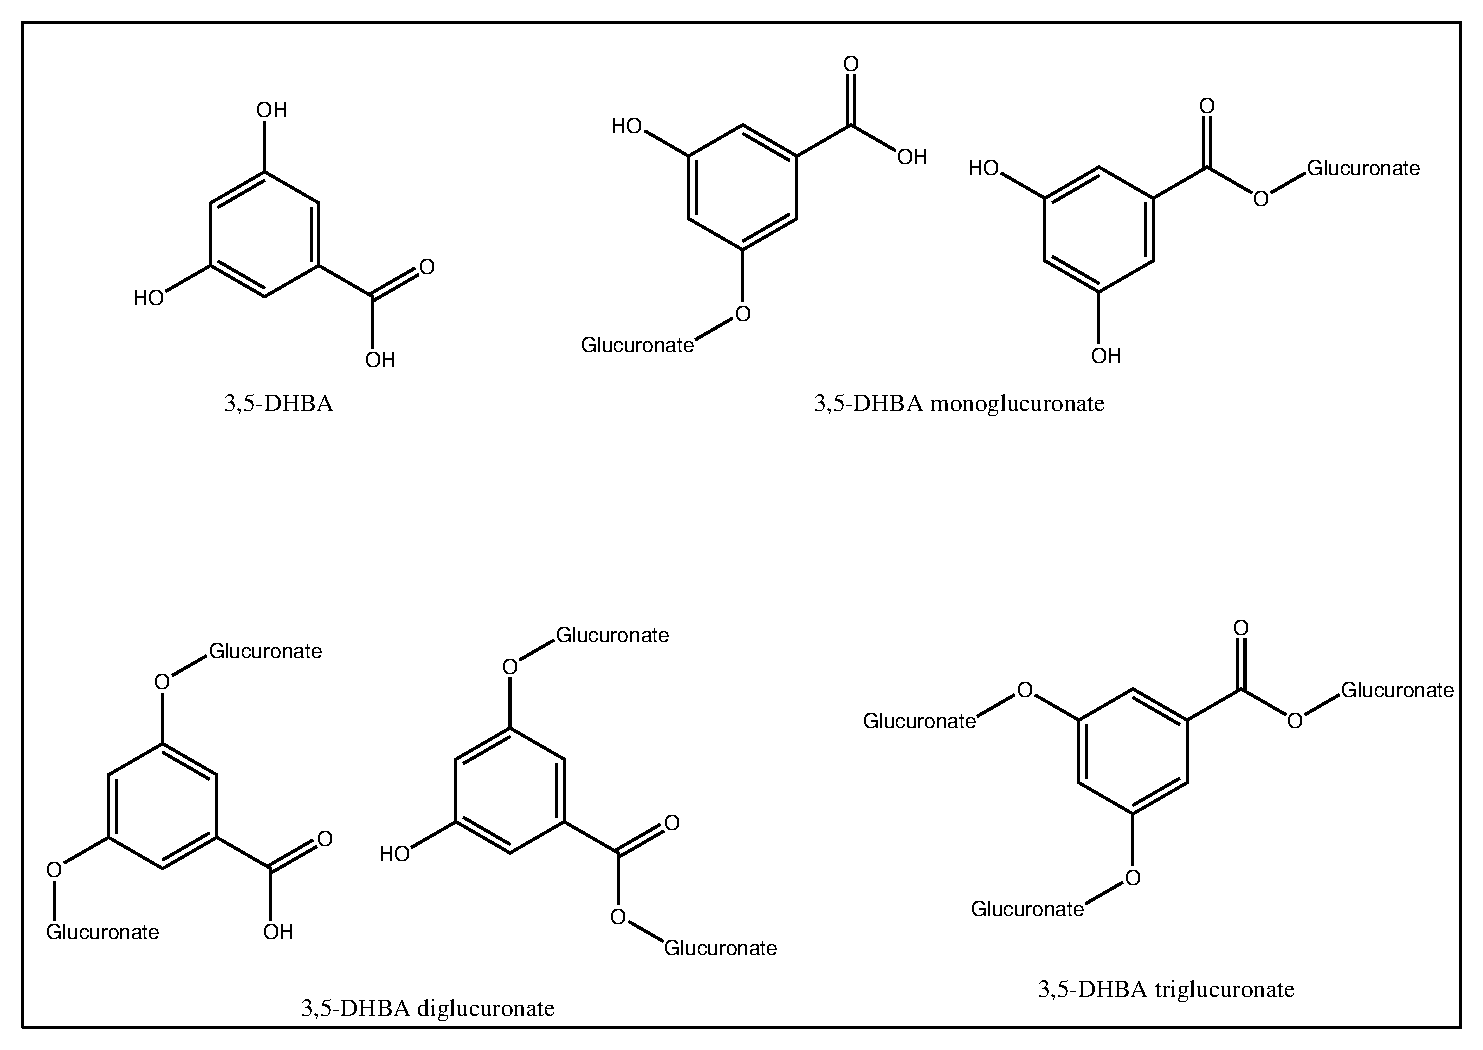
\includegraphics[width=1\linewidth]{picture/3,5-DHBA-glca-all}
	\caption{3,5-DHBA}
	\label{fig:35-dhba-all}
\end{figure}


\subsubsection{3,5-DHBA monoglucuronate}
3,5-DHBA mono-glucuronate exists 2 theoretical possibilities. Because position 3 and 5 are equal. The difference is phenol group or hydroxyl group sitting on carboxyl group be substituted.

Fragment 109 and 137 are specific for glucuronation reaction happening in carboxylic acid or beneze ring. Based on their predicted ClogP value and fragment 109 and 137 ratio. Finally, we confirmed RT 2.78 should be 3-glucuronate-5-hydroxyl-benzoic acid, RT 3.97 should be A. something in between, we have no idea.


\begin{figure}[h!]
	\centering
	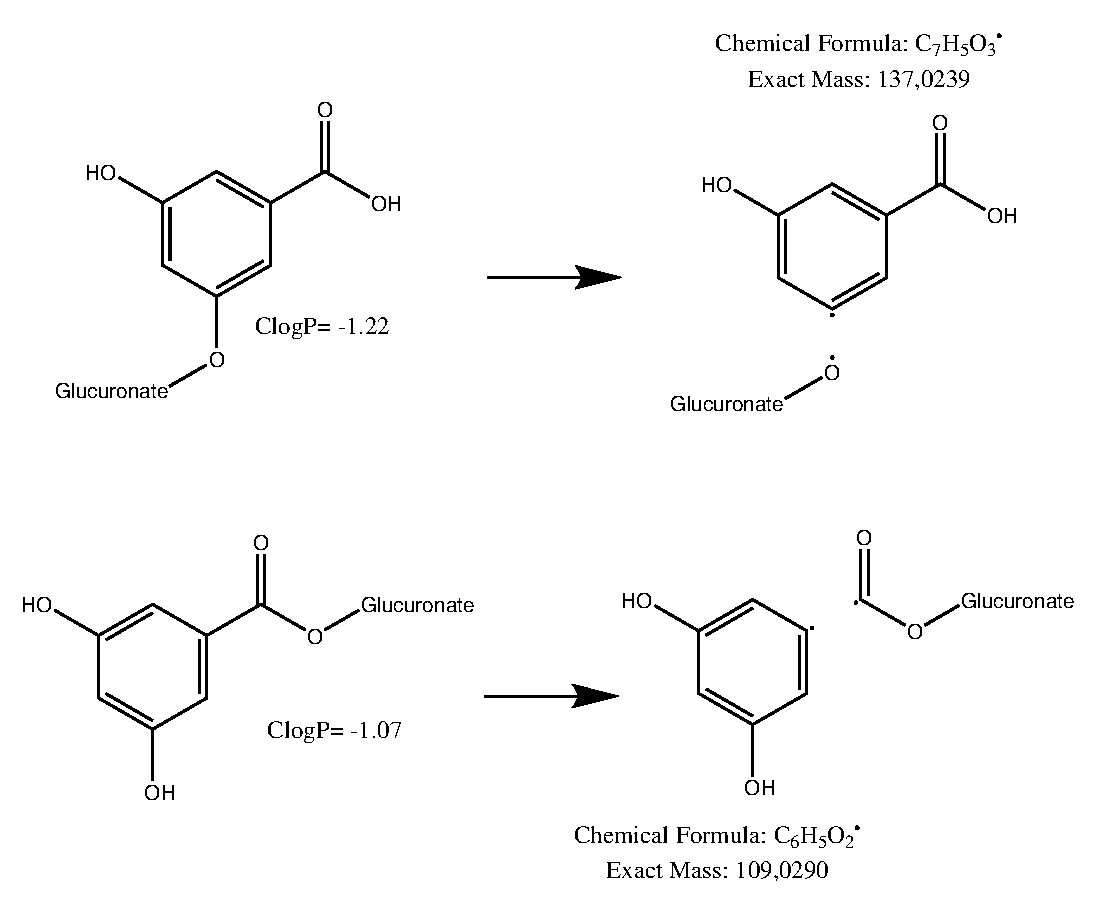
\includegraphics[width=1\linewidth]{picture/3,5-DHBA-glca-mono}
	\caption{Fragmentation of 3,5-DHBA monoglucuronate}
	\label{fig:35-dhba-glca-mono}
\end{figure}

\begin{table}[h!]
	\centering
\begin{tabular}{|c|c|c|c|}
	\hline 
	RT & \makecell{Intensity of\\ 109} & \makecell{Intensity of\\ 137} & \makecell{Ratio of \\109:137} \\ 
	\hline 
	2.78 & 195 & 1.58e3 & 1.23e-1 \\ 
	\hline 
	3.08 & 1.48e3 & 27.8 & 52.23 \\ 
	\hline 
	3.97 & 2.79e4 & 34.7 & 804 \\ 
	\hline 
\end{tabular} 
\caption{3,5-DHBA monoglucuronate}
\label{tab:35-dhba-monoglucuronate}
\end{table}

\subsubsection{3,5-DHBA diglucuronate and triglucuronate}
3,5-DHBA di- and tri- glucuronates were also detected.
3,5-DHBA di-glucuronate has 2 possible isomers. But they were not confirmed here.

3,5-DHBA tri-glucuronate does not have isomers. It is detected as [M+3 GluA-2H]2-.

\subsection{3,5-DHBA sulfate}

\subsection{Identifications of alkylresorcinol (AR) metabolites}

\section{Conclusion}


\section{Discussion}

%\chapter{Towards a Streamlined Metabolomics Data Analysis Flow: Unify Metabolomics Data Format Tidy}
%\section{Introduction}
Metabolomics data is characterized as high-dimension, storage space demanding.
In Metabolomics data analysis pipeline, normally different software will be included such as data preprocessing, statistics, annotation and visualization. Different software is programmed in different languages, such as R, java, MatLab or web-based applications.
Different software has different data storage format. This hurdles the data analysis workflow. Because a lot of time will be wasted in converting data format.
As estimated, in data analysis task, 70\% is spent in data preparing.
Therefore, reducing time spent in preparing different format, but focus more in its biological intrepertation will be promising.

\section{Materials and Methods}
We used R programming language, mainly use "tidyverse" package.

\section{Results}
m2r function: This function can convert Pls Toolbox (Eigenvector Research Inc.) to R tidy format.

c2r function: This function can convert MZmine converted '.csv' data to R tidy format.

\section{Discussions}
Definitely this software has a lot of shortcomings: 

\section{Conclusion}
Currently, lacks a bioinformatics tool intergrating all data format converting into one.
Our software can convert

%\chapter{Data Quality Control (QC) and Quality Assurance (QA) in LC-MS Based Untargeted Metabolomics}
%\begin{abstract}
	This is an abstract
\end{abstract}
Keywords:
\section{Introduction}


%\chapter{Several R Functions Facilitating LC-MS Based Metabolomics Data Analysis Workflow}
%\section{abstract}
	I would like to test whether it's possible to input an abstract here.,

\section{"Tidy" High-throughout Analysis Data, Examplified by RNA sequencing data}

\section{m2r}

\section{plot\_excretion}

\section{plot\_intervention}

%\chapter{Implementing A Streamlined Metabolomics Data Analysis Workflow (EZMS) Based on R Programming Language}

%\chapter{Using a Budgeted Device to Compute High-throughout Metabolomics Data}
%"MetaboPi"

\section{Abstract}
Handling high-throughout metabolomics data demands high computing and storage resource.  

How to compute the data locally (without sending it to a high-performance server) with a budgeted device could be an interesting topic to explore. 
Because this would provide possibilities to protect privacies in home-appliance or fulfil the real-time analysis tasks in some extreme conditions (such as in polar region or some areas with poor Internet connectivity)


why do i do this? because in the future, metabolomics analysis could become smart-home appliance, such as smart toilet or smart mirror. 
people can get their metabolome examined daily in their home.
such a good vision raised several problems. data privacy problem and cost.
because metabolome is considered as personal privacy. therefore, leak these privacy could result in bad results. however, if computed locally, whether it's possible to control the cost.

In this study, we simulated a computing task. 


Not only limited to human metabolome for risk analysis. it could also be applied in the fridge for example, to detect microorganisms' characteristic metabolome.

in less developed countries, or in portable devices, transmitting the data could be very expensive (via satalliate for example, in polar areas), therefore, computing such a dataset whether it's possible. 

\section{Introduction}
\subsubsection{Potential Use environment}
\subsubsection{hello}

\section{Solution}

\section{Business Model}
\chapter{Identification Strategies for BFIs Discovery}
\section{Introduction}
In this master thesis work, most of my time was spent on identifying metabolites from biospecies such as urine and plasma. This is same in all biomarker discovery studies. however, this step is very time-consuming. I summaried the identification strategies i used. This might be inspiring for other researchers.

In metabolimics pipeline, identification comes after statistics. Selected features (with retention time and mass-to-charge ratio) should be identified. 

\textbf{step one: database search}
Normally, 1st step starts from searching database. the database could be a public one or in-house one. Normally in-house database contains RT, fragments, adducts, etc. This might easily match get a level-one identification.
however, searching in a public database normally can get extensive hints, e.g. C6H10O might have a lot of hints.

\textbf{step two: use reference compound}
1st, reference compound is available. then purchase them, e.g. in my case, sitostanol did not fly in our Quad method. then, I checked another method, Linda's method to make it fly.

In another case, interesting compound could be an metabolite of the reference compound. Then, we need to some in-vitro metabolism experiments, e.g. oxidation, glucuronadation and sulfazation. If they match 

second method is, use glucuronadase or sulfatease to treat the sample and analyze them again, to check whether RT, m/z and MSMS spectra match.

Another challenge is reference compound is not always available. For example in Muyao's PhD thesis, she synthesized her own compound and made a level-1 identification for spinach intake.

\section{Materials and methods}
In order to identify researches dealing with the identification of BFIs, we carried out an extensive literature search following the BFIRev methodology proposed previously [4].
 Briefly, searches were carried out in three databases (PubMed, Scopus, and ISI Web of Knowledge) in Jun 2019. In PubMed, the search terms were (nutri- tion*[Title/Abstract]) AND (biomarker*[Title] OR marker*[Title]) AND (validation*[Title/Abstract] OR validity*[Title/Abstract] OR validate*[Title/Abstract] OR assessment*[Title/Abstract]) NOT (animal OR rat OR mouse OR mice OR pig) NOT (disease*[Title] OR risk*[- Title] OR inflammat*[Title/Abstract] OR patient*[Title]). To avoid all the studies concerned with a single bio- marker while keeping studies on validation in general, we avoided using nutrient* or food* in the search strat- egy. The fields used for the other two databases were [Article Title/Abstract/Keywords] for Scopus and [Topic] for ISI Web of Science to replace [Title/Ab- stract] for PubMed. The search was limited to papers in English language and with no restriction applied for the publication dates. The review papers discussing the de- velopment and application of biomarkers in the nutri- tion field were selected in the process outlined in Fig. 1. The first draft scheme of validation criteria was based on criteria proposed in the review papers found by this literature search. This list was revised by three rounds of commenting by co-authors as well as feedback from pre- sentations at international conferences.


\section{Discussion}
\subsection{Searching in a cohort study}
not all metabolites are identifiable. in order to prioritize the identification work, there's one step suggested before identification. That is, check whether this metabolite can also distinguish this intake in another large cohort study. Normally this is the later step of BFIs discovery study, i.e. validation of metabolites. 
However, these cohort studies normally do not share their data. Also because different analytical platform, data format was used making it difficult to compare.

\subsection{Challenges and Limitations}
Not enough.
normally they do not have bio-informatics ideas.


\chapter{Discussions}
I do not know which markers are better. If another dataset can give me. I think it's gonna be better.
%\addchap{Closing Remarks}
\end{document}
